\documentclass[tikz, border=6pt]{standalone}
\usepackage{tikz}
\usepackage{amsmath}
\usetikzlibrary{arrows.meta, positioning, calc, shapes.geometric, decorations.pathreplacing}

% ==============================================================================
% SECTION 4: DECOUPLED SUB-BLOCK GEOMETRY & COHABITATION
% 100% Unified Academic Palette Matching Section 5 Datapath & Section 7 FSM:
% Deepened "Batata" (#FEF08A) Fills + Crisp 2.2pt Black Outlines + High-Visibility Badges
% Expanded Vertical Architecture for Master Poster Scale (Aspect Ratio ~ 1.42)
% ==============================================================================
\definecolor{instBurgundy}{RGB}{112, 0, 24}      % #700018 Slot A / Type
\definecolor{instNavy}{RGB}{16, 44, 96}          % #102c60 Slot B / Marks
\definecolor{instCobalt}{RGB}{30, 58, 138}       % #1e3a8a Payload
\definecolor{instForest}{RGB}{4, 120, 87}        % #047857 Efficiency / Active
\definecolor{instSlack}{RGB}{100, 116, 139}      % #64748b Slack
\definecolor{batataFill}{HTML}{F5BC01}          % Rich Deepened "Batata" (#fef08a)
\definecolor{textDark}{HTML}{0F172A}            % Dark Slate Text (#0f172a)

\begin{document}
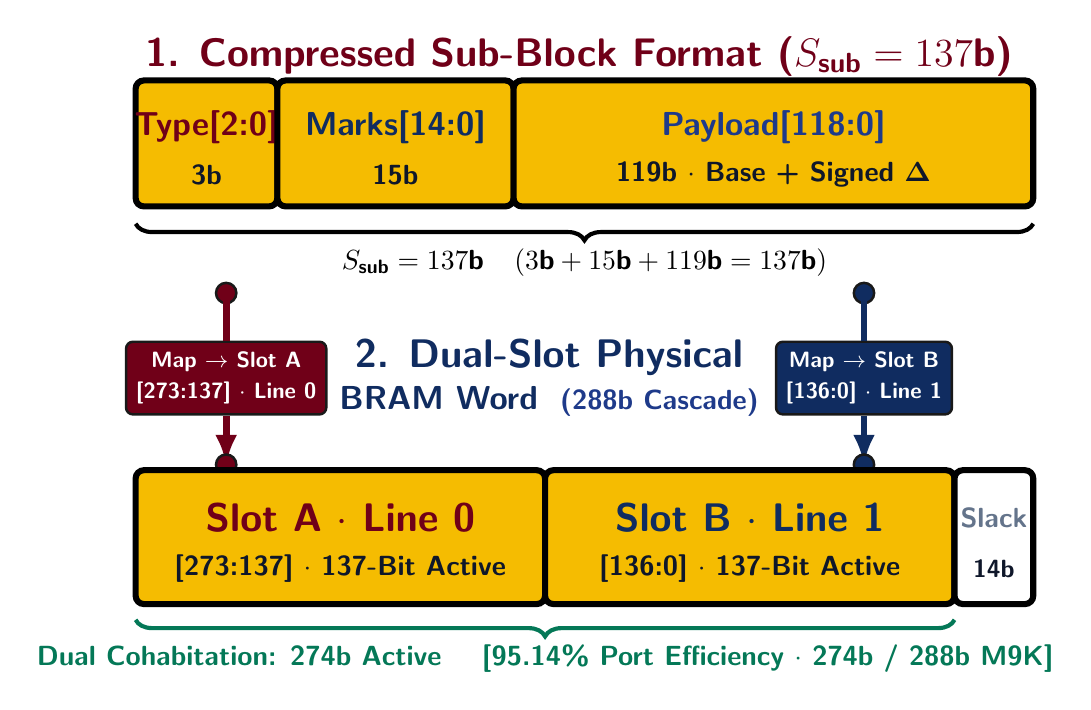
\begin{tikzpicture}[
    font=\sffamily,
    >=Latex,
    pDot/.style={circle, fill=#1, inner sep=2.6pt, draw=black!90!white, line width=0.9pt}
]

% ==============================================================================
% 1. TOP SECTION: 137-BIT COMPRESSED SUB-BLOCK (S_sub)
% ==============================================================================
\node[anchor=west, font=\sffamily\bfseries\Large, text=instBurgundy] at (0, 7.60) 
  {\textbf{1. Compressed Sub-Block Format} ($S_{\text{sub}} = 137\text{b}$)};

% Contiguous Sub-block fields: Deepened "Batata" (#FEF08A) Fill with Crisp Black 2.2pt Outlines
% Type[2:0]: 3b (x in [0, 1.8], y in [5.70, 7.30] -> Height: 1.6cm)
\draw[fill=batataFill, draw=black, line width=2.2pt, rounded corners=3pt] (0, 5.70) rectangle (1.8, 7.30);
\node[text=instBurgundy, align=center, font=\sffamily\bfseries\large] at (0.9, 6.70) {Type[2:0]};
\node[text=textDark, align=center, font=\sffamily\bfseries\normalsize] at (0.9, 6.10) {3b};

% Marks[14:0]: 15b (x in [1.8, 4.8], y in [5.70, 7.30] -> Height: 1.6cm)
\draw[fill=batataFill, draw=black, line width=2.2pt, rounded corners=3pt] (1.8, 5.70) rectangle (4.8, 7.30);
\node[text=instNavy, align=center, font=\sffamily\bfseries\large] at (3.3, 6.70) {Marks[14:0]};
\node[text=textDark, align=center, font=\sffamily\bfseries\normalsize] at (3.3, 6.10) {15b};

% Payload[118:0]: 119b (x in [4.8, 11.4], y in [5.70, 7.30] -> Height: 1.6cm)
\draw[fill=batataFill, draw=black, line width=2.2pt, rounded corners=3pt] (4.8, 5.70) rectangle (11.4, 7.30);
\node[text=instCobalt, align=center, font=\sffamily\bfseries\large] at (8.1, 6.70) {Payload[118:0]};
\node[text=textDark, align=center, font=\sffamily\bfseries\normalsize] at (8.1, 6.10) {119b $\cdot$ Base + Signed $\mathbf{\Delta}$};

% Sub-block Dimension Brace
\draw[decorate, decoration={brace, mirror, amplitude=6pt}, line width=1.5pt, color=black] 
    (0, 5.48) -- (11.4, 5.48) 
    node[midway, below=5pt, font=\sffamily\bfseries\normalsize, text=black] 
    {$S_{\text{sub}} = 137\text{b} \quad (3\text{b} + 15\text{b} + 119\text{b} = 137\text{b})$};

% ==============================================================================
% MAPPING ARROWS: DUAL COHABITATION PACKING (Solid 2.4pt Continuous Vectors)
% ==============================================================================
% Slot A Solid Mapping Arrow & Badge Pipeline (at x=1.15, drops from y=4.60 to y=2.42)
\node[pDot=instBurgundy] at (1.15, 4.60) {};
\node[fill=instBurgundy, text=white, draw=black!90!white, line width=0.9pt, font=\sffamily\bfseries\footnotesize, rounded corners=2.5pt, inner sep=3.6pt, align=center] 
  (badgeA) at (1.15, 3.52) {\textbf{Map $\to$ Slot A}\\[2pt]\textbf{[273:137] $\cdot$ Line 0}};
\draw[line width=2.4pt, color=instBurgundy] (1.15, 4.60) -- (badgeA.north);
\draw[->, line width=2.4pt, color=instBurgundy, >={Latex[length=3.8mm, width=2.8mm]}] (badgeA.south) -- (1.15, 2.42);
\node[pDot=instBurgundy] at (1.15, 2.42) {};

% Center Section 2 Header (Centered at x=5.25, with generous breathing space)
\node[align=center, font=\sffamily\bfseries, text=instNavy] at (5.25, 3.52) 
  {\Large\textbf{2. Dual-Slot Physical}\\[3.5pt] 
   \large\textbf{BRAM Word}\; \normalsize\textcolor{instCobalt}{\textbf{(288b Cascade)}}};

% Slot B Solid Mapping Arrow & Badge Pipeline (at x=9.25, drops from y=4.60 to y=2.42)
\node[pDot=instNavy] at (9.25, 4.60) {};
\node[fill=instNavy, text=white, draw=black!90!white, line width=0.9pt, font=\sffamily\bfseries\footnotesize, rounded corners=2.5pt, inner sep=3.6pt, align=center] 
  (badgeB) at (9.25, 3.52) {\textbf{Map $\to$ Slot B}\\[2pt]\textbf{[136:0] $\cdot$ Line 1}};
\draw[line width=2.4pt, color=instNavy] (9.25, 4.60) -- (badgeB.north);
\draw[->, line width=2.4pt, color=instNavy, >={Latex[length=3.8mm, width=2.8mm]}] (badgeB.south) -- (9.25, 2.42);
\node[pDot=instNavy] at (9.25, 2.42) {};

% ==============================================================================
% 2. BOTTOM SECTION: DUAL-SLOT PHYSICAL BRAM WORD (288b CASCADE)
% ==============================================================================
% Contiguous Physical Row: Deepened "Batata" (#FEF08A) Fill with Crisp Black 2.2pt Outlines
% Slot A: 137b (x in [0, 5.2], y in [0.65, 2.35] -> Height: 1.7cm)
\draw[fill=batataFill, draw=black, line width=2.2pt, rounded corners=3pt] (0, 0.65) rectangle (5.2, 2.35);
\node[text=instBurgundy, align=center, font=\sffamily\bfseries\Large] at (2.6, 1.75) {Slot A $\cdot$ Line 0};
\node[text=textDark, align=center, font=\sffamily\bfseries\normalsize] at (2.6, 1.10) {[273:137] $\cdot$ 137-Bit Active};

% Slot B: 137b (x in [5.2, 10.4], y in [0.65, 2.35] -> Height: 1.7cm)
\draw[fill=batataFill, draw=black, line width=2.2pt, rounded corners=3pt] (5.2, 0.65) rectangle (10.4, 2.35);
\node[text=instNavy, align=center, font=\sffamily\bfseries\Large] at (7.8, 1.75) {Slot B $\cdot$ Line 1};
\node[text=textDark, align=center, font=\sffamily\bfseries\normalsize] at (7.8, 1.10) {[136:0] $\cdot$ 137-Bit Active};

% Slack: 14b (x in [10.4, 11.4], y in [0.65, 2.35] -> Height: 1.7cm)
\draw[fill=white, draw=black, line width=2.2pt, rounded corners=3pt] (10.4, 0.65) rectangle (11.4, 2.35);
\node[text=instSlack, align=center, font=\sffamily\bfseries\normalsize] at (10.9, 1.75) {Slack};
\node[text=textDark, align=center, font=\sffamily\bfseries\small] at (10.9, 1.10) {14b};

% Active data brace under Slot A + Slot B
\draw[decorate, decoration={brace, mirror, amplitude=6pt}, line width=1.5pt, color=instForest] 
    (0, 0.45) -- (10.4, 0.45) 
    node[midway, below=5pt, font=\sffamily\bfseries\normalsize, text=instForest] 
    {Dual Cohabitation: 274b Active \quad [95.14\% Port Efficiency $\cdot$ 274b / 288b M9K]};

\end{tikzpicture}
\end{document}
